\documentclass[12pt,a4paper,oneside]{book}
\usepackage[english]{babel}
\usepackage{etex}
\usepackage{amsmath}
\usepackage{amsfonts}
\usepackage{graphicx}
\usepackage{amsmath}
\usepackage[utf8]{inputenc}
\usepackage{xcolor}
\usepackage{setspace}
\usepackage{float}
\usepackage{titlesec}
\usepackage{url}
\usepackage{wrapfig}
\usepackage[export]{adjustbox}
\usepackage[hidelinks]{hyperref}
\usepackage{anyfontsize}
\setcounter{tocdepth}{1}
\titleformat{\section}{\Huge\scshape\center}{}{0em}{}
\titleformat{\chapter}{\Huge\scshape\center}{}{0em}{}
\titleformat{\subsection}{\Large\scshape\raggedright}{}{0em}{} [{\titlerule[1pt]}]
\setlength\parindent{0pt}
\setlength{\parskip}{5pt}
\usepackage{fullpage}
\renewcommand\UrlFont{\rmfamily\itshape}
\font\myfont=cmr12 at 40pt
\begin{document}
\title{{\myfont My Cookbook}}
\author{{\Huge Author}}
\maketitle
\tableofcontents
\newpage

\part{Sample}
\chapter{Sample}

\newpage
\section{Sample}
\begin{center} \large Sample - Sample - Sample \end{center}
\subsection{Ingredients} 
\begin{minipage}{0.5\textwidth} 
\begin{itemize}
\item Sample 1
\item Sample 2
\end{itemize}
\end{minipage}
\begin{minipage}{0.5\textwidth}
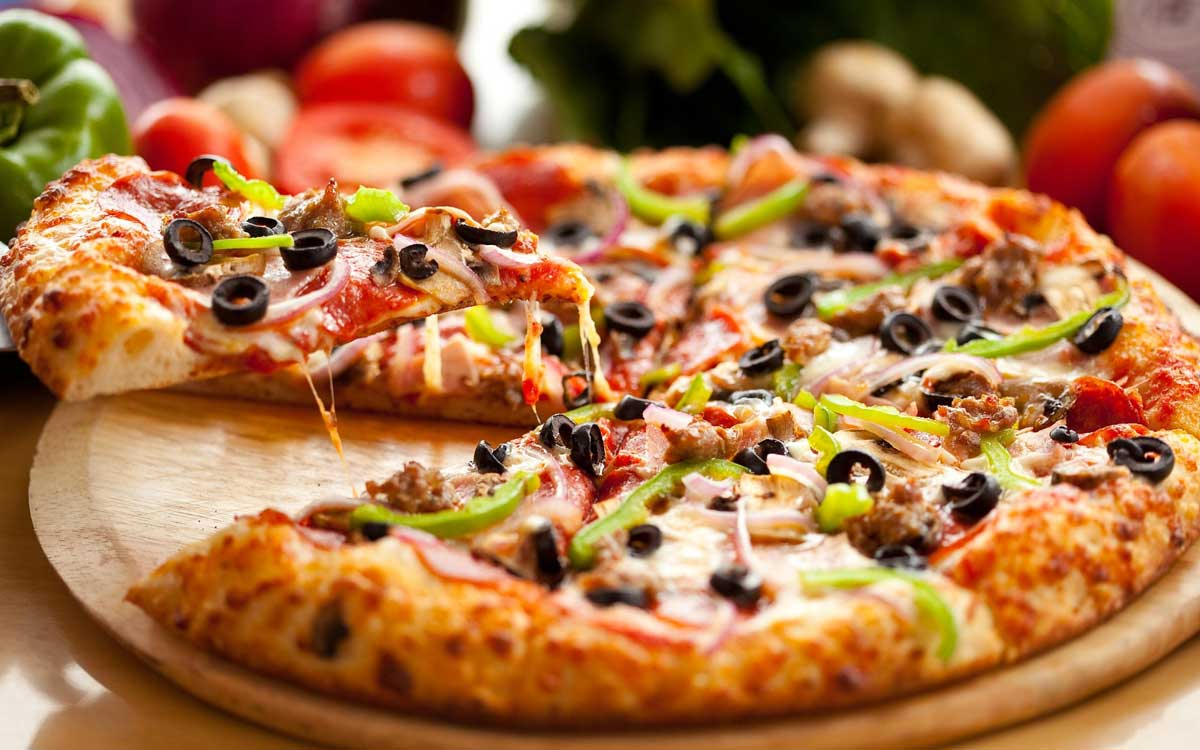
\includegraphics[width=0.9\linewidth]{pictures/c5dd1b2697720fe692c529688d3f4f8d.jpg}
\end{minipage}
\linespread{1.25}
\subsection{Steps}
\begin{itemize}
\item Sample 1.
\item Sample 2.
\end{itemize}

\end{document}